\chapter{Algorand}
\section{From Permissioned to Permissionless: Committee Selection}
Transitioning from a permissioned to a semi-permissionless setup involves addressing the challenge of selecting a committee of variable size ($N$) to execute a Byzantine Fault Tolerant (BFT) consensus protocol, such as HotStuff, in a distributed and verifiable manner. This committee, chosen based on the randomness of the previous block, plays a critical role in ensuring the safety and liveness of the protocol. If at least $\frac{2}{3}$ of the committee members are honest and online, the BFT protocol remains secure and operational. To account for randomness, a certain degree of slack is allowed in the honest committee member fraction. For instance, if the honest fraction is $0.7$, a $\frac{2}{3}$ honest supermajority within the committee can be achieved.\\
Directly selecting a fixed committee size is complex in a distributed context, but randomness can be introduced to determine the committee size, offering a viable alternative. This can be achieved using hash functions, similarly to the approach described in a previous lecture (Lecture 12). Each player, whether honest or malicious, participates in a lottery where they have a small probability of being elected. Consequently, the committee size ($N$) becomes random, albeit with a predictable expectation. For instance, if there are $700K$ honest players and $300K$ malicious ones in total, and the expected committee size is $E[N] = 1000$, each player's probability of being elected through the lottery is $0.001$. This results in the random variable $X$ following a Binomial($700K$, $0.001$) distribution, and similarly, another variable $Y$ follows Binomial($300K$, $0.001$), representing malicious committee members.\\
For a committee with a random size, two conditions are essential: 
\begin{enumerate}
	\item \textbf{Ensuring liveness:} $X \textgreater \frac{2E[N]}{3}$, guaranteeing that honest players can drive progress within the protocol.
	\item \textbf{Ensuring safety:}  $X + 2Y \textless \frac{4E[N]}{3}$, ensuring that the committee maintains a $\frac{2}{3}$ honest supermajority.
\end{enumerate}
Upon examining the probability distribution in this context (see figure \ref{fig:L16_f2}), it becomes evident that the likelihood of a random committee successfully executing a secure BFT protocol approaches certainty as the committee size and the number of participants increase.\\
However, this form of random committee selection faces security challenges due to potential attacks from adaptive adversaries. These vulnerabilities arise from two scenarios: 
\begin{itemize}
	\item Preknowledge of committee selection, allowing an adaptive adversary to preemptively corrupt committee members.
	\item Corrupting individual nodes within a committee during the BFT operation, compromising the protocol's integrity.
\end{itemize}
To mitigate these issues, Algorand introduces innovative solutions: 
\begin{itemize}
	\item A novel committee selection process that remains robust against adaptive adversaries, leveraging secret credentials.
	\item A novel BFT consensus mechanism that maintains robustness even when individual nodes within the committee are compromised.
\end{itemize}
These strategies are elaborated in subsequent sections, addressing the implementation of secure committee selection and BFT consensus protocols, as depicted in figure \ref{fig:L16_f3}b. Further insights into the execution of these solutions will be discussed in the upcoming sections.
\begin{center}
	\begin{figure}
		\centering
		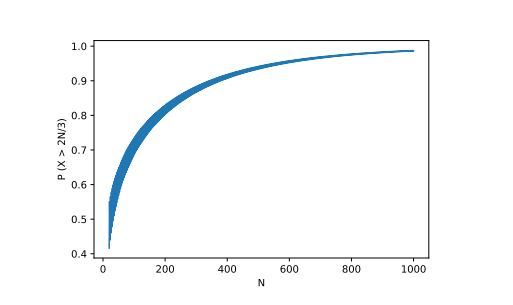
\includegraphics[width=0.8\linewidth]{Fig/16/F1}
		\caption{Probability of honest supermajority for fixed committee size $N$}
		\label{fig:f1}
	\end{figure}
\end{center}
\begin{center}
	\begin{figure}
		\centering
		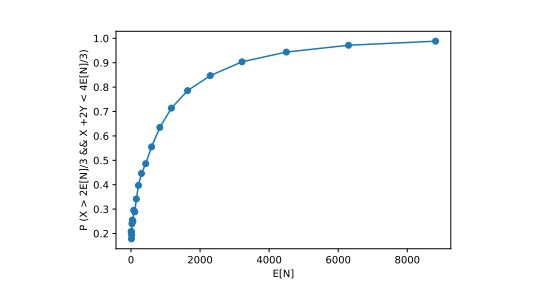
\includegraphics[width=0.8\linewidth]{Fig/16/F2}
		\caption{Probability of liveness and honest supermajority for a random committee size $N$. Total players $n = 1000000$ and honest fraction $0.7$. }
		\label{fig:L16_f2}
	\end{figure}
\end{center}
\begin{center}
	\begin{figure}
		\centering
		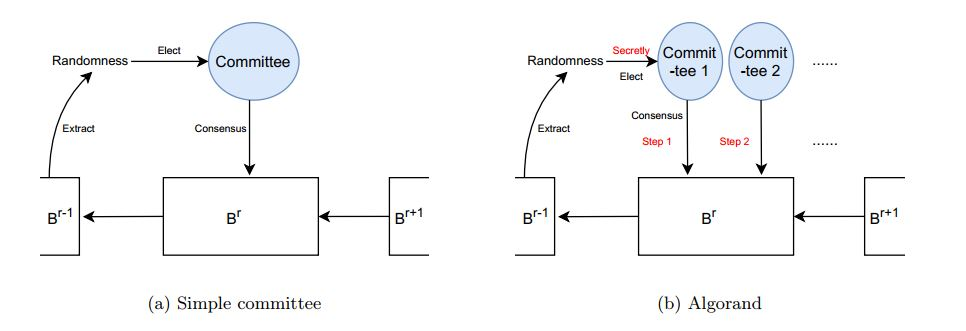
\includegraphics[width=0.8\linewidth]{Fig/16/F3}
		\caption{Simple committee selection vs Algorand committee selection}
		\label{fig:L16_f3}
	\end{figure}
\end{center}
\section{Player Replaceability and Secret Committee Election}
To counter the challenges posed by an adaptive adversary, Algorand introduces two fundamental properties: Player Replaceability and Secret Committee Election. These properties ensure the security and robustness of the Byzantine Fault Tolerant (BFT) protocol. Let's delve into how Algorand achieves these requirements.\\
Consider a scenario where we are executing a BFT protocol to determine the contents of block $B^{r}$ associated with round $r$. To ensure the randomness required for committee selection, a random quantity $Q^{r}$ is obtained from the previous block $B^{r-1}$ available on the blockchain. This randomness serves as a crucial element in generating secure and unbiased committee selections.\\
The BFT protocol for block $B^{r}$ involves multiple distinct steps, each identified by a step counter denoted as 's.' Algorand ensures that different committees are elected for each of these steps. To achieve this, the concept of a "credential" ($\alpha$) is introduced for player i during any committee selection stage. The credential $\sigma_{i}^{r, s}$ is derived in secret, utilizing the random quantity $Q^{r}$ and is a unique signature based on $r, s$, and $Q^{r}$. Specifically, if the result of the hash function H applied to $\alpha_{i}^{r, s}$ is less than a certain threshold value '$p$' $(H(\alpha_{i}^{r, s}) < p)$, then player $i$ is selected as a member of the committee for that step.\\
The unique secret signature is generated using Verifiable Random Functions (VRFs), which were introduced in Lecture 12. In this context, VRF($r, s, Q^{r}, sk_{i}$) $<$ $p$ is used to generate the signature, where $sk_{i}$ represents the private key for the VRF. The threshold value '$p$' is carefully chosen to ensure an appropriate expected committee size.\\
As the BFT protocol progresses and it becomes time for player $i$ to participate in step 's,' player i includes their credential $\alpha_{i}^{r, s}$ with their message. Other players can then verify this inclusion, even if player $i$ is maliciously corrupted. Importantly, the message cannot be prevented from reaching other honest players. Furthermore, any influence the adversary might gain from corrupting a player is limited; they have no more control over the protocol's progression than they would have by corrupting a randomly chosen player.\\
This process of secret committee election, utilizing credentials and VRFs to generate verifiable signatures, effectively achieves Player Replaceability. Each substep of the BFT protocol has its own randomly and independently selected committee, making the protocol resistant to preknowledge-based attacks. This ensures that an adaptive adversary cannot exploit committee predictability or corrupt members preemptively. The innovative combination of Player Replaceability and Secret Committee Election fortifies Algorand's BFT protocol against adaptive adversaries, preserving the protocol's security and integrity.
\subsection{Ephemeral keys}
To counter the potential threat of an adaptive adversary who could corrupt committee members after learning their identities, Algorand employs a mechanism known as ephemeral keys. These keys are one-time-use public/secret key pairs that provide an added layer of security against the adversary's tactics.\\
Here's how ephemeral keys work within Algorand's framework:
\begin{enumerate}
	\item \textbf{Generation of Ephemeral Key Pairs:} For each player-round-step triple ($i, r, s$), player $i$ generates a master key pair. This master key pair is then used to generate ephemeral key pairs for multiple rounds and steps. Importantly, once these ephemeral key pairs are generated and used, the master secret key is destroyed to prevent any future use. The master public key, however, is made public.
	\item \textbf{Ephemeral Key Usage:} During round $r$, step $s$, if player $i$ is elected as a committee member, they use the ephemeral key pair specifically generated for the ($i, r, s$) triple to sign messages relevant to that committee participation. Once these messages are signed, the ephemeral secret key is destroyed. It's worth noting that ephemeral keys are only used to sign messages, while the long-term public/secret key pairs are reserved for signing credentials $\alpha$.
	\item \textbf{Contrast with Key Evolving Scheme (KES):} Ephemeral keys differ from the key evolving scheme (KES) introduced in Lecture 12. In KES, keys evolve from the previous ephemeral key pair, while in the case of ephemeral keys in Algorand, they are generated by a master key pair. The ephemeral key pairs used for a specific ($i, r, s$) triple are destroyed after use, and a player does not need to retain keys for every round and step unless elected as a committee member.
\end{enumerate}
The use of ephemeral keys provides an additional level of protection against adaptive adversaries. By generating new keys for each committee participation and destroying them afterward, Algorand ensures that even if the adversary identifies committee members based on their messages, they cannot corrupt those members and coerce them into certifying a fake block. This mechanism enhances the security of Algorand's protocol and ensures that the integrity of the consensus process is upheld while also being efficient and well-suited for the permissionless setting.

\section{Algorand: Single Round BFT Consensus Protocol}
We commence with a probabilistic binary Byzantine Fault Tolerant (BFT) consensus protocol that lacks the characteristic of player replaceability. However, it inherently allows for the integration of this feature, as we will elucidate subsequently.\\
The primary objective of this protocol is to facilitate consensus among a total of $n = 3t + 1$ players, where $t$ represents the threshold for tolerating Byzantine faults. Each individual player, denoted as $i$, possesses a binary value $b_{i}$ as their input, which they aim to reconcile. Throughout the course of the protocol, participants continuously update their local binary value $b_{i}$ based on the information received. Upon conclusion, the protocol strives for a unanimous output among honest players, signifying that they should converge to the same binary value $b$. If all honest players initially hold the same input value, implying there exists a value $b$ such that $b_{i} = b$ for every honest player, the protocol's objective is for them to eventually output the same value $b$, i.e., $b_{i} = b$ remains valid for all honest players.
The protocol operates within synchronized steps, where the delivery of messages is ensured to occur within a designated step. Therefore, the protocol's design aligns with that of a synchronous network, akin to the mechanics of the longest chain protocol. Each step follows the paradigm below:\\
\begin{table}[htbp]
	\centering
	\begin{tabular}{|>{\centering\arraybackslash}p{4cm}|>{\centering\arraybackslash}p{8cm}|}
		\hline
		Start of a step & End of a step\\
		\hline
		Every player propagates $b_{i}$ & Every player updates $b_{i}$ based on the received messages\\
		\hline
	\end{tabular}
\end{table}
\section{Consensus On a Binary Value}
Algorand's binary Byzantine Fault Tolerant (BFT) consensus protocol operates in a perpetual loop, systematically cycling through three distinct steps. The protocol's structure is depicted in Figure \ref{fig:L16_f4}, and it employs a counter variable denoted as "$s$" (initiated at $s = 1$) to signify the number of executed steps. Consequently, the first step corresponds to $s = 1, 4, ...$, the second step to $s = 2, 5, ...$, and the third step to $s = 3, 6, ...$.\\
The first and second steps of the protocol adhere to the previously discussed property (A). Additionally, they are designed to ensure that once consensus has been attained regarding a specific bit, an honest participant can discern this achievement, output the corresponding bit, and conclude their involvement. This property is formally articulated as property (C).\\
(C) If an honest player "$i$" outputs a value during the first or second step, then the protocol guarantees that consensus will prevail by the end of that step. Moreover, the third step embodies both property (A) and (B), as previously detailed. By leveraging these properties, the protocol's nature as a Byzantine consensus protocol is established. Specifically, properties (A) and (C) work together to prevent honest players from outputting disparate values, while properties (A) and (B) ensure the eventual convergence and output of a unanimous value, thereby culminating in an agreement.
\begin{center}
	\begin{figure}
		\centering
		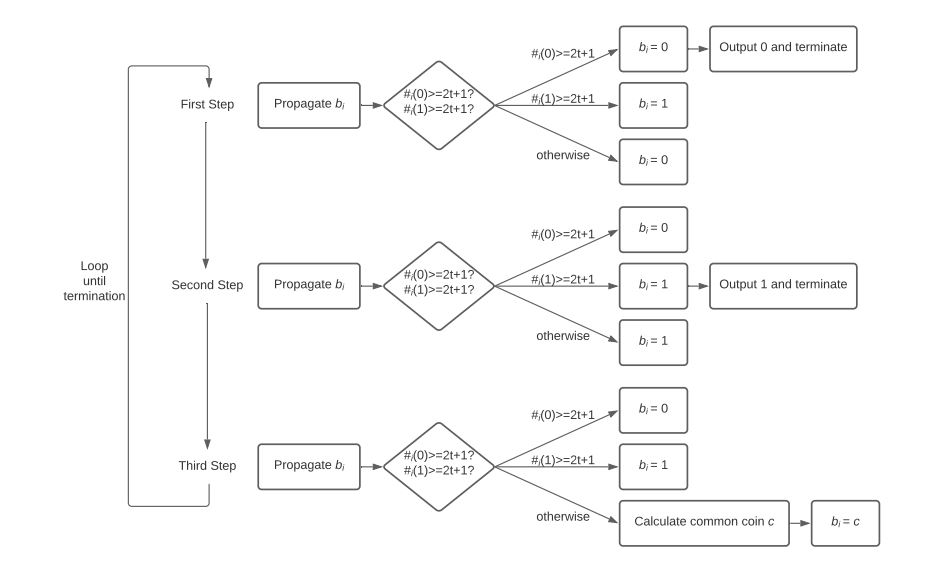
\includegraphics[width=0.8\linewidth]{Fig/16/F4}
		\caption{Algorand consensus on a binary value}
		\label{fig:L16_f4}
	\end{figure}
\end{center}
\section{Adding Player Replaceability And Secret Committee Election}
Incorporating the committee into the protocol involves granting message propagation eligibility exclusively to committee members. However, it's important to note that the fundamental process of updating the local value "$b_{i}$" remains a shared responsibility among all players. The overall communication complexity is now quantified as $O(nN)$, attributable to each committee member transmitting messages to every player.\\
The introduction of player replaceability and secret committee election hinges on the computation of credentials, as elucidated in the previous section. Upon calculating its credential for a specific round "$r$" and step "$s$" (denoted as $\alpha_{i}^{r, s}$), a player discerns its role within the committee and is equipped with the means to substantiate this role. This substantiation is achieved by appending the calculated credential to its messages during the respective step.\\
In the protocol diagram depicted in Figure \ref{fig:L16_f4}, a simple adaptation is necessary: the parameter "$2t + 1$" is replaced with "$\frac{2E[N]}{3}$." This change is necessitated by the fact that the random committee now boasts an anticipated size of $E[N]$ rather than the original fixed size of $n = 3t + 1$.
\section{Multivalue Consensus}
Extending the Algorand consensus from binary values to multivalued scenarios involves the election of a leader for each round "r," responsible for constructing and distributing a valid block denoted as $B^{r}$. The process of electing the "potential leader" remains analogous to the committee election, albeit with a significantly smaller threshold. This adjustment leads to the selection of only a few dozen players as potential leaders.\\
Once potential leaders are identified, they proceed to propagate their respective blocks. Each player evaluates potential leaders and selects the leader whose credential hash is the smallest. Subsequently, they cast their vote for the block hash twice, with the second vote being dispatched only if the first vote receives more than two-thirds of first-vote responses.\\
After the block proposing and two-round voting stages, each player reaches one of two conditions: either (a) they receive a valid block $B^{r}$ from the leader along with sufficient votes for its hash, or (b) no valid block garners enough votes for its hash.\\
In the case of condition (a), player $i$ initiates the binary protocol with an initial value $b_{i} = 0$. Conversely, in condition (b), the initial value is set to $b_{i} = 1$." During the binary protocol, players append the block hash to their messages, ensuring alignment on the held block in condition (a). The two-round voting process further guarantees consensus among honest players in condition (a), ensuring agreement on the same block $B^{r}$.\\
The binary protocol's outcome provides essential insights: a value of $0$ signifies the finalization of block $B^{r}$, which is universally acknowledged. Conversely, a value of $1$ signifies the finalization of an empty block $B_\epsilon^{r}$.\\
It's worth noting that the block proposing and two-round voting steps, akin to previous stages, remain both committee-based and player-replaceable. This overarching approach imbues the entire Algorand protocol with committee-based dynamics and the flexibility of player replaceability.
\section{Conclusion}
In the Algorand consensus protocol, players collectively agree on the contents of each block $B_{r}$ for round $r$. The Algorand Blockchain is constructed by executing the consensus protocol round by round, sequentially generating blocks $B^{1}$, $B^{2}$, and so on, with each block containing a hash pointer to its parent block $B_{r}$. Each round involves communication complexity of $O(nN)$ and concludes within a constant expected number of steps, as detailed in previous sections.\\
Algorand can also be adapted into a proof-of-stake (PoS) blockchain by factoring in the stake held by a public key during the committee/leader election process. A higher stake increases the likelihood of being elected. Importantly, Algorand's inherent resistance to forking mitigates issues such as key grinding and nothing-at-stake attacks that plague other PoS mechanisms, as seen in the longest chain version of PoS.\\
However, Algorand's security model is predicated on a synchronous network setting, where messages are guaranteed to be delivered within a step.\\
It's important to note that while Algorand offers robust security, there exists a potential weakness related to forensics. In a scenario where the number of Byzantine players exceeds the threshold $t$, these malicious actors can deviate from the protocol and trigger a safety violation. Unlike some other consensus algorithms, such as HotStuff or Streamlet, Algorand may experience a safety attack that doesn't leave behind cryptographic evidence. For instance, if a significant fraction of Byzantine players abstains from sending votes during the second step, they can cause an honest player majority to switch their local value, leading to a safety breach. Importantly, since these Byzantine players don't send any messages, there's no cryptographic evidence to hold them accountable.\\
This forensics challenge persists in Algorand regardless of the inclusion of committee elections and player replaceability. The question of whether an efficient BFT protocol with strong forensic support and player replaceability can serve as a core consensus engine within a PoS permissionless blockchain remains an open research question.

\renewcommand{\bibname}{References}
\begin{thebibliography}{9}
	\bibitem{reference1} Silvio Micali. Byzantine agreement, made trivial, 2018.
	\bibitem{reference2} Jing Chen and Silvio Micali. Algorand: A secure and efficient distributed ledger. \textit{Theoretical Computer Science, 777:155183, 2019}.
	\bibitem{reference3} Peiyao Sheng, Gerui Wang, Kartik Nayak, Sreeram Kannan, and Pramod Viswanath. Bft protocol forensics, 2020.
\end{thebibliography}